
%(BEGIN_QUESTION)
% Copyright 2014, Tony R. Kuphaldt, released under the Creative Commons Attribution License (v 1.0)
% This means you may do almost anything with this work of mine, so long as you give me proper credit

Explain, step by step, how to calculate the amount of current ($I$) that will go through each resistor in this parallel circuit, and also the current ($I$) supplied by the DC voltage source:

$$\includegraphics[width=15.5cm]{i01237x01.eps}$$

\underbar{file i01237}
%(END_QUESTION)





%(BEGIN_ANSWER)

First we need to identify all the relevant principles for series circuits:

\begin{itemize}
\item{} The algebraic sum of all currents at a node will be equal to zero (Kirchhoff's Current Law)
\item{} Voltage is common throughout a parallel circuit, because every component shares the same two equipotential points
\item{} Resistances diminish in parallel
\end{itemize}

Following from the rule that voltage is common throughout a parallel circuit, we may conclude that each of the three resistors sees 36 volts from the source.  Thus, we may immediately apply Ohm's Law to calculate current through each of the resistors, knowing the voltage across each resistor and the resistance of each resistor:

$$I_{R1} = {V \over R_1} = {36 \hbox{ V} \over 1500 \> \Omega} = 24 \hbox{ mA}$$

$$I_{R2} = {V \over R_2} = {36 \hbox{ V} \over 10000 \> \Omega} = 3.6 \hbox{ mA}$$

$$I_{R3} = {V \over R_3} = {36 \hbox{ V} \over 4700 \> \Omega} = 7.660 \hbox{ mA}$$

It is helpful to annotate all calculated values on the circuit schematic for easy reference.  The reason this is helpful is because it applies a context to the calculated value.  Here we will sketch arrows (in the direction of conventional flow) to document all three resistor currents, based on the relationship between voltage and current for {\it loads} (i.e. current enters the positive pole of a load because the load is opposing that current):

$$\includegraphics[width=15.5cm]{i01237x02.eps}$$

\filbreak

From here we may apply KCL to calculate current values at the each node, knowing that every milliamp leaving a node must be matched by a milliamp of current entering the node.  Current entering the upper-right node, therefore, will be the sum of the two currents exiting that node.  The same thing happens at the lower-right node, where two currents entering that node merge to form a larger current exiting:

$$I = 3.6 \hbox{ mA} + 7.660 \hbox{ mA} = 11.260 \hbox{ mA}$$

Once again we will document this calculated value on the circuit schematic to maintain its context:

$$\includegraphics[width=15.5cm]{i01237x03.eps}$$

Applying KCL to the upper-left and lower-left nodes, and annotating the schematic once again:

$$I = 24 \hbox{ mA} + 11.260 \hbox{ mA} = 35.260 \hbox{ mA}$$

$$\includegraphics[width=15.5cm]{i01237x04.eps}$$

With the arrows showing this 35.260 mA current, we can see it passes straight out of (and back in to) the 36 volt source, which means this is our total current value for the parallel circuit.

%(END_ANSWER)





%(BEGIN_NOTES)


%(END_NOTES)


